\documentclass[11pt,a4paper]{report}

\usepackage{minted}
\usepackage{extarrows}
\usepackage{graphics}
\usepackage{enumitem}

\usepackage{colortbl}
\usepackage{tabularx}

\usepackage{wrapfig}
\usepackage{multirow}

\usepackage{mathdots}
%\usepackage{amsmath}
\usepackage{amssymb}
\usepackage{amsfonts}
\usepackage{mathrsfs}
\usepackage{mathtools}

\usepackage{fancyhdr}
\usepackage{makeidx}
 
%\usepackage{color}
\usepackage[dvipsnames]{xcolor}
\usepackage{graphicx}
\usepackage{epstopdf}
\usepackage{multicol}

\usepackage{hyperref}
\usepackage{geometry}

\usepackage{soul}
\usepackage{xfrac}
% \newcommand{\sout}[1]{#1}

\usepackage{combelow}

\usepackage{array}

\usepackage[T1]{fontenc}
\usepackage[utf8]{inputenc}

\definecolor{bg}{gray}{0.96}
\definecolor{codegreen}{rgb}{0,0.6,0}
\definecolor{codegray}{rgb}{0.5,0.5,0.5}
\definecolor{codepurple}{rgb}{0.58,0,0.82}

\usepackage{showexpl}
\lstdefinestyle{ourstyle}{
    backgroundcolor=\color{bg},   
    commentstyle=\color{codegreen},
    keywordstyle=\color{magenta},
    numberstyle=\tiny\color{codegray},
    stringstyle=\color{codepurple},
    basicstyle=\ttfamily\footnotesize,
    texcsstyle=*\color{codepurple},
    breakatwhitespace=false,         
    breaklines=true,                 
    captionpos=b,                    
    keepspaces=true,                 
    numbers=left,                    
    numbersep=5pt,                  
    showspaces=false,                
    showstringspaces=false,
    showtabs=false,                  
    tabsize=2,
}
 
\lstset{language=[LaTeX]Tex,
  style=ourstyle,
}

\newenvironment{example5}%
  {\VerbatimEnvironment
    \begin{VerbatimOut}{tmp/eqnexample.tmp}}%
    {\end{VerbatimOut}%
    \noindent
    \begin{minipage}{0.5\textwidth}%
    \latexFile{tmp/eqnexample.tmp}%
    \end{minipage}
    \begin{minipage}{0.5\textwidth}\setlength{\parindent}{0.5cm}%
    \input{tmp/eqnexample.tmp}%
    \end{minipage}%
  }
  
\newenvironment{examplefr}%
  {\VerbatimEnvironment
    \begin{VerbatimOut}{tmp/eqnexample.tmp}}%
    {\end{VerbatimOut}%
    \noindent
    \latexFile{tmp/eqnexample.tmp}%
    \input{tmp/eqnexample.tmp}%
  }
\newenvironment{examplef}%
  {\VerbatimEnvironment
    \begin{VerbatimOut}{tmp/eqnexample.tmp}}%
    {\end{VerbatimOut}%
    \noindent
    \begin{minipage}{\textwidth}%
    \latexFile{tmp/eqnexample.tmp}%
    \end{minipage}
    \begin{minipage}{\textwidth}\setlength{\parindent}{0.5cm}%
    \input{tmp/eqnexample.tmp}%
    \end{minipage}%
  }
\newenvironment{example}%
  {\VerbatimEnvironment
    \begin{VerbatimOut}{tmp/eqnexample.tmp}}%
    {\end{VerbatimOut}%
    \noindent
    \begin{minipage}{0.6\textwidth}%
    \latexFile{tmp/eqnexample.tmp}%
    \end{minipage}
    \begin{minipage}{0.4\textwidth}\setlength{\parindent}{0.5cm}%
    \input{tmp/eqnexample.tmp}%
    \end{minipage}%
  }


%\definecolor{bg}{HTML}{F0F0F0}
\newmintinline[code]{latex}{bgcolor=bg,
}
\newminted[latex]{latex}{bgcolor=bg,
}
\newmintedfile[latexFile]{latex}{bgcolor=bg,
  %linenos,
  %frame=rightline
}
%\newenvironment{example}{\begin{LTXexample}}{\end{LTXexample}}

%\renewcommand{\code}[1]{\verbclstinlineode{#1}}

%\newcommand{\coden}[1]{\ceo texttt{#1}}
%\newcommand{\coden}[1]{\lstinline{#1}}
\newcommand{\coden}[1]{\code{#1}}
\newcommand{\keyword}[1]{\coden{#1}}

\newcommand{\codeshowD}[2]{\coden{#1} & $#1$ & \coden{#2} & $#2$}
\newcommand{\codeshowB}[3]{\coden{#1} & $\displaystyle#1$ &
\coden{#2} & $\displaystyle #2$ &
\coden{#3} & $\displaystyle #3$\\}

\newcommand{\package}[1]{\code{\usepackage{#1}}\label{#1}}
\newcommand{\noncurs}{\hspace{.5cm}$\notin \mathscr{C}$}


\newcommand{\mtshow}[1]{\code{#1} & $#1$ \\}
\newcommand{\dmtshow}[1]{\code{#1} & $\displaystyle #1$ \\}

\newcommand{\explain}[2]{\code{#1} & #1 & #2\\}
\newcommand{\explainC}[2]{\code{#1} & #1 & #2 &}
\newcommand{\justexplain}[2]{\code{#1} & #2\\}
\newcommand{\explainM}[2]{\code{#1} & $#1$ & #2\\}

\newcommand{\explainMFont}[2]{\explainM{#1 {ABC\ i\ abc\ 123}}{#2}}
\newcommand{\explainMFontUpper}[2]{\explainM{#1 {ABC\ I\ DEF}}{#2 (uppercase only)}}

\newcommand{\codeshow}[1]{\code{#1} - #1}
\newcommand{\mcodeshow}[1]{\code{#1} - $#1$}
\newcommand{\dmcodeshow}[1]{\code{#1} - $\displaystyle #1$}
\newcommand{\codeeg}[1]{e.g. \codeshow{#1}}

\newcommand{\packageSubsection}[2]{\subsection[#1]{#1 - \code{#2}}}
\newcommand{\subsubsectionNoncurs}[1]{\subsubsection[#1]{#1 \noncurs}}
\newcommand{\subsectionNoncurs}[1]{\subsection[#1]{#1 \noncurs}}
\newcommand{\sectionNoncurs}[1]{\section[#1]{#1 \noncurs}}
\newcommand{\note}[1]{\textbf{Note:} #1}

%\usepackage[romanian]{babel}

\geometry{a4paper,left=25mm,right=20mm,top=20mm,bottom=30mm}

\newcommand{\book}{\code{book}\ }
\newcommand{\article}{\code{article}\ }
\newcommand{\report}{\code{report}\ }

\hypersetup{colorlinks=true, linkcolor=Blue, citecolor=green,
  filecolor=black, urlcolor=blue}
\usepackage{longtable} % To display tables on several pages

\renewcommand{\indexname}{I\lowercase{ndice}}

\usepackage{amsthm}
\renewcommand*{\proofname}{\noindent\textbf{Demonstra\c{t}ie.}}
\renewcommand{\qedsymbol}{$\blacksquare$}

\theoremstyle{plain} %the default style
\newtheorem{theo}{Teorema}
\newtheorem{corol}[theo]{Corolarul}
\newtheorem{prop}{Propozi\c{t}ia}[section]
\theoremstyle{definition}
\newtheorem{defin}{Defini\c{t}ia}[section]
\newtheorem{exem}{Exemplul}[section]

\renewcommand{\bibname}{Bibliografie}

\title{\LaTeX{} Cheatsheet}
\author{Łucasz Zieliński\thanks{Dzięki światu}}
\date{\today}

\newcommand*{\R}{\mathbb{R}}
\makeindex
%%%%%%%%%%%%%%
\begin{document}
%\begin{titlepage}
%\maketitle
%\end{titlepage}

\tableofcontents
%\listoffigures


\chapter{Das gute Zeug}
\section{Document classes \& differences}
\code{\documentclass[...]{report, article, book, beamer}}\\
e.g. \code{\documentclass[11pt,a4paper]{report}}

\subsection*{Differences with regard to available commands and environments}
\begin{itemize}\setlength{\itemsep}{0mm}
\item \book and \report feature the \code{\chapter} sectioning command, while \article doesn't.
\item In \book and \report, \code{\appendix} will cause \code{\chapter}s to be typeset as ``Appendix X'' instead of ``Chapter X''. For article, this isn't applicable.
\item \book and \report will start a new page for \code{\part}s , while \article won't.
\item \book offers the \code{\frontmatter}, \code{\mainmatter}, and \code{\backmatter} commands to control page numbering (Roman for the front matter, arabic elsewhere) and numbering of sectioning titles (no numbering in the front and back matter), while \report and \article don't.
\item \book \textit{doesn't} offer the \code{abstract} environment, while \report and \article \textit{do}.
\end{itemize}
\subsection*{Differences with regard to default settings}
\begin{itemize}\setlength{\itemsep}{0mm}
  \item The \book class uses the \code{twoside} class option (which means different margins and headers/footers for even and odd pages), while \report and \article use \code{oneside}.
  \item The \book class uses the \code{twoside} class option (which means different margins and headers/footers for even and odd pages), while \report and \article use \code{oneside}.
  \item \book uses \code{openright} (new parts and chapters start on ``right'' pages, adding a blank page before if necessary), while \report uses \code{openany}. (Note that ``right'' means an odd page in twoside mode, but any page in oneside mode.) For \article, the distinction between \code{openright} and \code{openany} isn't applicable.
    
  \item \book uses the \code{headings} pagestyle for non-chapter-starting pages, while \report and \article always use \code{plain}.
    
  \item \book and \report use \code{titlepage} (the title page and -- if applicable -- the \code{abstract} environment will be typeset on pages of their own), while \article uses \code{notitlepage}.
    
  \item For \book and \report, the lowest-level sectioning command which is numbered and incorporated into the table of contents is \code{\subsection}, while for article it is \code{\subsubsection}.
    
  \item \book and \report will use the arguments of \code{\chapter}s and \code{\section}s for running headings (if such headings are present), while \article will use \code{\section}s and \code{\subsection}s.
    
  \item \book and \report will number floats (figures, tables etc.), equations, and footnotes per chapter, while \article will number them continuously. Note that footnotes -- even when numbered per chapter -- do not feature a chapter prefix.

  \item \book and \report will use \code{\bibname} (which defaults to ``Bibliography'') for the heading of bibliographic references, while article will use \code{\refname} (which defaults to ``References'').
\end{itemize}

\section{Packages}
\subsection{Math}
\begin{latex}
\usepackage{amsmath} % adds a lot of math stuff 
\usepackage{mathtools} % fixes some amsmath things and adds more
\usepackage{amssymb} % adds a lot of math symbols 
\usepackage{amsfonts} % stuff like \mathbb
\usepackage{mathrsfs} % for \mathscr
\end{latex}

\subsection{Colors}
\begin{latex}
\usepackage{color}
%or even better (adds names like \RoyalPurple)
\usepackage[dvipsnames]{xcolor}
\end{latex}
\subsubsection* {Defining colors}
\code{\definecolor{name}{HTML}{RRGGBB}}, we can could also use \code{rgb} or \code{gray} instead of
\code{HTML}.

The option \texttt{[dvipsnames]} from \code{xcolor} defines PascalCase color names like in css like
'\code{MidnightBlue}'.

\subsubsection{Using colors}
\codeshow{\colorbox{blue}{fundal}}\\
\codeshow{\fcolorbox{Black}{White}{text}} - \code{\fcolorbox{margine}{fundal}{text}}\\
\code{\pagecolor{White}}\\
or \codeshow{\color{red} hello \color{black}}\\
or \codeshow{{\color{red} hello}}

\subsection{Images}
\begin{latex}
%preable
\usepackage{graphicx}
\usepackage{epstopdf}% for eps images

%in document
\includegraphics[scale=.4, angle=45]{something}
\includegraphics[width=3cm, height=4cm]{something}
\includegraphics[width=0.5\textwidth]{something}
\end{latex}
Tell where the images are, relative to main \texttt{.tex} file:\\
\code{\graphicspath}\texttt{\{ \{./images/\} \{./images2/\} \}}

\subsection{Figure}\label{figure}
\begin{latex}
\begin{figure}[!hbt]
  \includegraphics[width=\textwidth]{plot}
  \caption{Caption}\label{plot}
\centering
\end{figure}
\end{latex}
\note{You can use \code{wrapfigure} for wraping text around a figure.
  See \nameref{wraptable}} (page \pageref{wraptable}).
Options:
\begin{longtable}{l l}
  \justexplain{h}{place here - kinda}
  \justexplain{h!}{place here - more strict}
  \justexplain{t}{top of the page}
  \justexplain{b}{bottom of the page}
  \justexplain{p}{on a special page}
\end{longtable}

Two figures inline:
\begin{latex}
\begin{figure}[!hbt]
  \centering
  \includegraphics[height = 3cm]{stema.eps}
  \hspace{3cm}
  \includegraphics[width = 3cm]{Escher_Relativity.jpg}
  \caption[Imagini\^{i}n linie]{Stema Facult\u{a}\c{t}ii de Matematic\u{a}
    \c{s}i \textit{Relativitate} de M.C. Escher (1953)}\label{Stema_Escher2}
\end{figure}
\end{latex}

\note{We can use minipages to number them separately.}

To number them separately but within the same main number use \code{subfigure} 
(Requires the package \code{subfigure}):
\begin{latex}
\begin{figure}[!htb]
  \centering
  \subfigure[Stema Facult\u{a}\c{t}ii de Matematic\u{a}]{
    \includegraphics[height=3cm]{stema.eps}\label{Stema4}}
  \hspace{3cm}
  \subfigure[\textit{Relativitate} de M.C. Escher (1953)]{
    \includegraphics[width=3cm]{Escher_Relativity.jpg}\label{Escher4}
  }\\
  \caption{Stema Facult\u{a}\c{t}ii de Matematic\u{a}
    \c{s}i \textit{Relativitate} de M.C. Escher (1953)}\label{Stema_Escher4}}
\end{figure}
\end{latex}
\subsection{Fancy quotes \& Unicode}
\begin{latex}
\usepackage[T1]{fontenc}
% allows inserting unicode directly in latex (i.e. from keyboard)
\usepackage[utf8]{inputenc} % \noncurs
\end{latex}

\begin{longtable}{l c l}
\explain{\quotesinglbase}{Single low-9 quotation mark}
\explain{\quotedblbase}{Double low-9 quotation mark}
\explain{\guillemetleft}{Left-pointing double angle quotation mark}
\explain{\guillemetright}{Right-pointing double angle quotation mark}
\explain{\guilsinglleft}{Single left-pointing angle quotation mark}
\explain{\guilsinglright}{Single right-pointing angle quotation mark}
\explain{'}{Single high quotation mark}
\explain{`}{Single high-6 quotation mark}
\explain{``}{Double high-6 quotation mark}
\explain{''}{Double high-9 quotation mark}
\explain{"}{Double high-straight quotation mark}
\end{longtable}

\begin{example}
\begin{center}
\quotedblbase Cze\'s\'c'' czy ,,dzien dobry''. \\
\textquotedblleft Hello\textquotedblright{} 
or ``Hi''.\\
\guillemetleft Bonjour\guillemetright{}.
\end{center}
\end{example}

\subsection{Centering and setting font sizes}
Quick Usage:
\begin{latex}
\usepackage{sectsty}
\chaptertitlefont{\centering\LARGE}
\sectionfont{\Large}
\end{latex}

Long list (tl;dr - executes ... before printing whatever it says): \noncurs
\vspace{-11pt}
\begin{multicols}{2} \noindent
  \code{\allsectionsfont{...}} \\
  \code{\partfont{... }}\\
  \code{\chapterfont{...}}\\
  \code{\sectionfont{...}}\\
  \code{\subsectionfont{...}}\\
  \code{\subsubsectionfont{...}}\\
\columnbreak
  \code{\paragraphfont{...}}\\
  \code{\subparagraphfont{...}}\\
  \code{\minisecfont{...}}\\
  \code{\partnumberfont{...}}\\
  \code{\parttitlefont{...}}\\
  \code{\chapternumberfont{...}}\\
  \code{\chaptertitlefont{...}}
\end{multicols}

\subsection{Links and references}
\begin{latex}
\usepackage{hyperref}
\hypersetup{colorlinks=true, linkcolor=cyan, citecolor=green,
  filecolor=black, urlcolor=blue}
\end{latex}
More in \nameref{labels} (page \pageref{labels})

\subsection{Dots after chapters in table of contents}
\package{tocloft}\\
\code{\renewcommand{\cftchapleader}{\cftdotfill{\cftdotsep}}}

If we are in \article, we use:\\
\code{\renewcommand{\cftsecleader}{\cftdotfill{\cftdotsep}}}

\note{if this command is misspelled the error doesn't appear immediately,
but when a chapter is added to the Table of Contents.}


\section{Environments}

\subsection{Text alignment}

%\begin{center} \code{\begin{center} ... \end{center}}  \end{center}
%\begin{flushleft} \code{\begin{flushleft} ... \end{flushleft}} \end{flushleft}
%\begin{flushright} \code{\begin{flushright} ... \end{flushright}} \end{flushright}

\code{\begin{center} Centered \end{center}} \\
\code{\begin{flushleft} Left \end{flushleft}} \\
\code{\begin{flushright} Right \end{flushright}}

\subsection{Mini Page} %http://www.sascha-frank.com/latex-minipage.html
Useful for putting things side by side
\subsubsection{Usage}
\begin{latex}
\begin{minipage}[adjusting]{width of the minipage}
 Text | Images | ... 
\end{minipage} 
\end{latex}
\subsubsection{Adjustment}
When adjusting the choices is: \coden{c} (centers), \coden{t} (top) and \coden{b} (bottom).
By default, \coden{c} is used for centering. It is aligned by \code{t} and/or \code{b}
at the highest (top line) and/or at the lowest line (bottom line).
\subsubsection{Further options}
Besides there are still further options, which however in practical application the minipage does not play a role like the height and the adjustment (again \coden{c}, \coden{t} and \coden{b}) within the minipage.

Example of further options:
\code{\begin{minipage}[t][5cm][b]{0,5\textwidth}}

  This minipage now has a defined height of 5cm, and the content will now be aligned to the bottom of the minipage.
\subsubsection{Hint}

A mistake that is often made is, there is a blank line between the \code{\end{minipage}} and
\code{\begin{minipage}} left. Then the pages are no longer together.
  
\subsubsection{Example}
\begin{latex}
\begin{minipage}[t]{0.3\textwidth}
  \includegraphics[width=\textwidth]{pic1}
\end{minipage}

\end{latex}

\subsection{Others}
For \coden{abstract}, \coden{titlepage}, \coden{thebibliography}, see
\nameref{docStructure} (page \pageref{docStructure}).

For math stuff, see \nameref{math}\footnote{Natürlich}.

\section{Romanian Names and diacritics}
\subsection[Quick way]{Quick way \noncurs}

\code{\usepackage[romanian]{babel}}

\subsection{Long way}
\begin{latex}
\renewcommand{\contentsname}{Cuprins}
\renewcommand{\chaptername}{Capitolul}

\renewcommand{\bibname}{B\lowercase{ibliografie}}
\renewcommand{\refname}{B\lowercase{ibliografie}} %in article

\renewcommand{\appendixname}{Anexa}
\renewcommand{\indexname}{I\lowercase{ndice}}
\renewcommand{\abstractname}{Rezumatul lucr\u{a}rii}
\renewcommand{\listtablename}{Lista de tabele}
\renewcommand{\listfigurename}{Lista de figuri}
\end{latex}

\note{don't combine The Long way with The Quick way.}

\subsectionNoncurs{Proper diacritics}
\package{combelow}\\
\codeshow{\cb{s} \cb{t}, not \c{s} \c{t}}\\
Easier diacritics:
\begin{latex}
\code{\usepackage[romanian]{babel}}
\useshorthands{'}
\defineshorthand{'t}{\cb{t}}
\end{latex}

\sectionNoncurs{Macro definitions}
\begin{latex}
  \newcommand{\mat}[1]{\mathcal{M}_{#1}(\mathbb{R})}
% this "*" makes it that it complains if a \par is encountered
\newcommand*{\dx}[1][x]{\, \mathrm{d}#1}
\renewcommand{\contentsname}{Cuprins}


\usepackage{xparse}
% O, o optional, m= mandatory
\DeclareDocumentEnvironment{problema}{O {1} o m}{
  \begin{enumerate}[leftmargin=*]
    \addtocounter{enumi}{#1}
    \item
}{
  \end{enumerate}
  \IfValueT{#2}{\cppcode{#2}}
}
\newenvironment{\name}{begin}{end}

\end{latex}

Using \code{\renewcommand} inside an environment will make that definition local 
to the environment.

\note{remember to add "\code{\\}" before the command name (ie. not \code{\newcommand{foo}{}})}

\section{Fancy Headers}
\subsection{Main Commands}

\begin{latex}
\pagestyle{fancy}
\thispagestyle{fancy} % only for one page
\lhead{\nouppercase{\leftmark}}
\chead{\chaptername}
\rhead{\rightmark}
\lfoot{\thechapter}
\cfoot{\thepage}
\rfoot{\thesection}

\fancyhf{} % reset the fancy settings
\end{latex}

\subsection{Page Styles}

\begin{longtable}{l m{13cm}}
\justexplain{empty}{Both header and footer are cleared}
\justexplain{plain}{Header is clear, but the footer contains the page number in the center}
\justexplain{headings}{Footer is blank, header displays information according to document class (e.g., section name) and page number top right.}
\justexplain{myheadings}{Page number is top right, and it is possible to control the rest of the header.}
\end{longtable}

The commands \code{\markright} and \code{\markboth} can be used to set the content
of the headings by hand.The following commands placed at the beginning of an article
document will set the header of all pages (one-sided) to contain ``John Smith'' top
left, ``On page styles'' centered and the page number top right:
\begin{latex}
\pagestyle{headings}
\markright{John Smith\hfill On page styles\hfill}
\end{latex}

\subsection{Information commands}
There are special commands containing details on the running page of the document.
\begin{longtable}{l m{13cm}}
\justexplain{\thepage}{number of the current page}
\justexplain{\leftmark}{current chapter (or section for articles) name printed like ``CHAPTER 3. THIS IS THE CHAPTER TITLE''}
\justexplain{\rightmark}{current section (or subsection for articles) name printed like ``1.6. THIS IS THE SECTION TITLE''}
\justexplain{\chaptername}{the name chapter in the current language. If this is English, it will display ``Chapter''}
\justexplain{\thechapter}{current chapter number}
\justexplain{\thesection}{current section number}
\end{longtable}

Example:
\begin{examplefr}
\renewcommand{\chaptermark}[1]{ \markboth{#1}{} }
\renewcommand{\sectionmark}[1]{ \markright{#1}{} }
\pagestyle{fancy}
\cfoot{Page - \thepage}
\lhead{L Mark - \nouppercase{\leftmark}}
\rhead{R Mark - \nouppercase{\rightmark}}
\chead{C Name - \chaptername}
\lfoot{The Chapter - \thechapter}
\rfoot{The Section - \thesection}
\end{examplefr}

Note that \code{\leftmark} and \code{\rightmark} convert the names to uppercase, whichever was the formatting of the text. If you want them to print the actual name of the chapter without converting it to uppercase use the following command: 

\begin{latex}
\renewcommand{\chaptermark}[1]{ \markboth{#1}{} }
\renewcommand{\sectionmark}[1]{ \markright{#1}{} }
\end{latex}

Now \code{\leftmark} and \code{\rightmark} will just print the name of the chapter and section, without number and without affecting the formatting.
Note that these redefinitions must be inserted \emph{after} the first call of \code{\pagestyle{fancy}}. The standard book formatting of the \code{\chaptermark} is:
\begin{latex}
\renewcommand{\chaptermark}[1]{\markboth{
    \MakeUppercase{\chaptername\ \thechapter.\ #1}}{}}
\end{latex}
Moreover, with the following commands you can define the thickness of the decorative lines on both the header and the footer:
\begin{latex}
\renewcommand{\headrulewidth}{0.5pt}
\renewcommand{\footrulewidth}{0pt}
\end{latex}

\subsection{\texttt{fancyhdr}}
Add this in your preamble:
\begin{latex}
\usepackage{fancyhdr}
\setlength{\headheight}{15.2pt}
\pagestyle{fancy}
\end{latex}

You can use these commands to customize headers and footers
\begin{latex}
\lhead[<even output>]{<odd output>}
\chead[<even output>]{<odd output>}
\rhead[<even output>]{<odd output>}

\lfoot[<even output>]{<odd output>}
\cfoot[<even output>]{<odd output>}
\rfoot[<even output>]{<odd output>}
\end{latex}

Example:
\begin{latex}
\lhead[Author Name]{}
\rhead[]{Author Name}
\lhead[]{\today}
\rhead[\today]{}
\lfoot[\thepage]{}
\rfoot[]{\thepage}
\end{latex}

\subsection[\texttt{titlesec}]{\texttt{titlesec} - not tested \noncurs}
Useful for showing first thing on page - not last.
\begin{latex}
\usepackage[pagestyles]{titlesec}
% Definition of the page style with required headers
\newpagestyle{TitleMarks}{%
  \sethead[Top is~\toptitlemarks\thesubsection]% even-left
    [First is~\firsttitlemarks\thesubsection]% even-center
    [Bottom is~\bottitlemarks\thesubsection]% even-right
    {Top is~\toptitlemarks\thesubsection}% odd-left
    {First is~\firsttitlemarks\thesubsection}% odd-center
    {Bottom is~\bottitlemarks\thesubsection}% odd-right
}
\end{latex}

\subsection{Page \emph{n} of \emph{m}}
\begin{latex}
\usepackage{lastpage}
...
\cfoot{\thepage\ of \pageref{LastPage} }
\end{latex}
\fancyhf{}
\lhead{\nouppercase{\leftmark}}
\rhead{\nouppercase{\rightmark}}
\cfoot{\thepage}
\vspace{-1cm}
\section{References and labels}\label{labels}
Requires \package{hyperref}.

\subsection{Labels}
\codeshow{\label{aLabel}}\\
\codeshow{\ref{aLabel}}\\
\codeshow{\ref*{aLabel}}\\
\codeshow{\nameref{aLabel}}\\
\codeshow{\nameref*{aLabel}}\\
\codeshow{\pageref{aLabel}}\\
\codeshow{\autoref{aLabel}}\\
\codeshow{\hyperref[aLabel]{here}}\\
% \codeshow{\hyperref{aLabel}}
\codeshow{\url{run:/usr/bin/firefox}}\\
\codeshow{\href{run:/usr/bin/firefox}{here}}\\
\codeshow{\cite{author/19}}\\
\codeshow{\cite[Chapter IV]{author/19}}\\
\codeshow{\eqref{aLabel}}

Adding "*" to \code{\...ref} will not create a clickable thing (the text is black).

Not adding \code{\phantomsection} before a link or reference might not center the page properly\\
e.g. \code{\phantomsection\label{bLabel}}


\subsection{Web Links}
\codeshow{\href{http://example.com/}{here}}\\
\codeshow{\url{http://example.com/}}\\
\codeshow{\href{mailto:my_addr@a.com}{my\_addr@a.com}}\\
\code{\nolinkurl} makes it so \LaTeX{} doesn't complain about an invalid url\\
\codeshow{\href{mailto:my_addr@a.org}{\nolinkurl{my_addr@a.org}}}

\subsection{Settings}
Using \code{\usepackage[hidelinks]{hyperref}} will make links black.
\subsubsection{Short way}
\begin{latex}
\hypersetup{colorlinks=true, linkcolor=cyan, citecolor=green,
  filecolor=black, urlcolor=blue}
\end{latex}
\subsubsectionNoncurs{Full way}
\begin{latex}
\hypersetup{
    bookmarks=true,         % show bookmarks bar?
    unicode=false,          % non-Latin characters in Acrobat’s bookmarks
    pdftoolbar=true,        % show Acrobat’s toolbar?
    pdfmenubar=true,        % show Acrobat’s menu?
    pdffitwindow=false,     % window fit to page when opened
    pdfstartview={FitH},    % fits the width of the page to the window
    pdftitle={My title},    % title
    pdfauthor={Author},     % author
    pdfsubject={Subject},   % subject of the document
    pdfcreator={Creator},   % creator of the document
    pdfproducer={Producer}, % producer of the document
    pdfkeywords={keyword1, key2, key3}, % list of keywords
    pdfnewwindow=true,      % links in new PDF window
    colorlinks=false,       % false: boxed links; true: colored links
    linkcolor=red,          % color of internal links
    citecolor=green,        % color of links to bibliography
    filecolor=magenta,      % color of file links
    urlcolor=cyan,          % color of external links
    %if colorlinks=false:
    linkbordercolor={1 0 0},% color of frame around internal links
    citebordercolor={0 1 0},% color of frame around citations
    urlbordercolor={0 1 1}  % color of frame around URL links
}  
\end{latex}
\note{The explicit RGB specification is only allowed for the border colors (like linkbordercolor etc.), while the others may only assigned to named colors.}
\section{Footnotes}
\subsection{Usage}
\codeshow{Text\footnote{hi there} more text.}

To use whatever number:\\
\codeshow{\footnote[9]{fn 2}}

To define footnote style:\\
\codeshow{\renewcommand{\thefootnote}{\roman{footnote}}}\footnote{like so} or\\

\codeshow{\renewcommand{\thefootnote}{\fnsymbol{footnote}}\footnote{fn 4}}\\
\renewcommand{\thefootnote}{\arabic{footnote}}

Reset footnotes:\\
\codeshow{\setcounter{footnote}{0}}

For continuous footnotes:\\
\package{chngcntr}


\subsection{Number footnotes continuously in all chapters}
In \book and \report footnotes are reset every chapter, to number them continuously do this:\\
\code{\counterwithout{footnote}{chapter}}\footnote{Requires the package \code{chngcntr}}

\subsection{Forcing footnotes when it doesn't work}
In math mode\footnote[19]{but not in the \code{equation} environment} and tables
\code{\footnote} doesn't work.\\
Instead use: \code{\footnotemark[18] ... \footnotetext[18]{hi}}.
\\
\begin{example5}
\begin{tabular}{l l}
  bar\footnotemark & I'm a table \\
  baz\footnotemark & Very tabley\\
\end{tabular}
\footnotetext{Now shown}\\
\end{example5}

\note{Using multiple \code{\footnotemark}s might not number them properly}\\
\codeeg{\footnotetext{Now shown 2}}

  

\pagestyle{plain}
\chapter{Math}\label{math}
\section{Math mode}
\begin{itemize}
\item \textbf{Inline} can be entered by using \code{$...$} or \code{\(...\)}, or by using
  the environment \code{math}
\item \textbf{Displayed} mode can be entered using \code{\[...\]} or with the environment
  \code{displaymath}.\\
  Using the environment \code{equation} automatically numbers the equation.\\
  \code{equation*} and \code{displaymath} are functionally equivalent
\end{itemize}
\codeeg{\[F(x) = \int f(x)\, dx \]}\\
\codeeg{$F(x) = \int f(x)\,dx$}

\note{Adding \code{fleq} in the \code{\documentclass} options aligns equations to the left}

Most spaces are ignored, and must be specified manually.
\note{LaTeX complains if you leave empty lines in math mode.}

Adding \code{\numberwithin{equation}{section}} will reset equation numbers every section.
\code{chapter} may also be used.

\subsection{Bold Math}
\begin{example}
  this doesn't work: \textbf{Text $f$}\\
  this works: \textbf{Text} $\boldsymbol{f}$
\end{example}
\subsection{Font size}
\begin{longtable}{l l }
  \code{\displaystyle} & $\displaystyle \int$\\
  \code{\textstyle} & $\textstyle \int$\\
  \code{\scriptstyle} & $\scriptstyle \int$\\
  \code{\scriptscriptsyle} & $\scriptscriptstyle  \int$
\end{longtable}

Declaring \code{\everymath{\displaystyle}} in the preamble will force \code{\displaystyle}
in all math environments



\section{Environments}
\note{Adding \code{\nonumber} to an otherwise numbered environments cancels the numbering.}\\
\note{Adding more white space than needed inside \code{align} and \code{aligned} makes latex complain.}

Since ``a picture is worth a thousand words'', just look at this:

\subsection{align}
Writing \code{\allowdisplaybreaks} in the preamble allows splitting an equation written in \code{align} on multiple pages.

\begin{example}
\begin{align}
  a & = 3\\
    & = 2 + 1 \nonumber \\
    & = 2 + \sigma(0)
\end{align}
\end{example}

Adding small interjections to align:\\
\begin{example}
\begin{minipage}{3in}
\begin{align*}
\intertext{If}
   A &= \sigma_1+\sigma_2\\
   B &= \rho_1+\rho_2\\
\intertext{then}
C(x) &= e^{Ax^2+\pi}+B
\end{align*} 
\end{minipage}
\end{example}

\subsection{aligned}
Like align but used inside math mode. Useful for numbering multiple lines once.

\begin{example}
\begin{equation}
\begin{aligned}
  a & = 3\\
    & = 2 + \sigma(0)
\end{aligned}
\end{equation}
\end{example}

\subsection{eqnarray}
People on the internet say ``don't use \code{eqnarray}'' so we won't talk about it.

\subsection{subequations}
\begin{example}
\begin{subequations}
\begin{align}
  a &= 3\\
  &= 2 + \sigma(0)
\end{align}
\end{subequations}
\end{example}

or:

\begin{example}
\begin{subequations}
\begin{equation}
  a = 3\label{blasphemy}
\end{equation}
Therefore:
\begin{equation}
  \int_0^1\sqrt{1-x^2} dx = \frac{3}{4}
\end{equation}
\end{subequations}

The equation \eqref{blasphemy} %(\ref{blasphemy})
is obviously false\footnote{
  Unless you are an engineer}.
\end{example}


\subsection{cases}
Useful for functions with multiple branches.

\begin{example}
\[f(x) =
\begin{cases}
  \int\frac{\sin(x)}{x},&\text{daca } x \neq 0,\\
  1,&\text{daca } x=0.
\end{cases}
\]
\end{example}

With displaystyle:\\
\begin{example}
\[f(x) =
\begin{dcases}
  \int\frac{\sin(x)}{x},&\text{daca } x \neq 0,\\
  1,&\text{daca } x=0.
\end{dcases}
\]
\end{example}

If there's a lot of plain text on the right\footnote{same goes for \code{cases*}}:\\
\begin{example}
\[f(x) =
  \begin{dcases*}
    \int \frac{\sin(x)}{x},&daca $x \neq 0$,\\
    1,& daca $x=0$.
  \end{dcases*}
\]
\end{example}


\newcommand{\parti}[2]{\frac{\partial #1}{\partial #2}}
Nice spacing:\\
\begin{example}
%\newcommand{\parti}[2]{\frac{\partial #1}
%  {\partial #2}}
\[f(x, y) =
\begin{dcases}
  \parti{g}{x}\,,&\text{daca } x y \geq 0,\\[0.5em]
  \parti{g}{y}\,,&\text{daca } x y < 0,
\end{dcases}
\]
\end{example}

vs\\
\begin{example}
\[f(x, y) =
\begin{dcases}
 \parti{g}{x},&\text{daca } x y \geq 0,\\
 \parti{g}{y},&\text{daca } x y < 0,
\end{dcases}
\]
\end{example}



\subsection{matrix}
For writing matrices with more columns (default is 10):
\code{\setcounter{MaxMatrixCols}{15}}

\begin{tabular}{|l|l|}
  \hline
  Environment name & Surrounding delimiter\\
  \hline
pmatrix & $( )$\\
bmatrix & $[ ]$\\
Bmatrix & $\{ \}$\\
vmatrix & $| |$\\
Vmatrix & $\Vert \Vert$\\
  \hline
\end{tabular}

\begin{example}
\[
A_{m,n} = 
 \begin{pmatrix}
  a_{1,1} & a_{1,2} & \cdots & a_{1,n} \\
  a_{2,1} & a_{2,2} & \cdots & a_{2,n} \\
  \vdots  & \vdots  & \ddots & \vdots  \\
  a_{m,1} & a_{m,2} & \cdots & a_{m,n} 
\end{pmatrix}
\]
\end{example}

Nicer spacing:\\
\begin{example}
\begin{equation*}
  \begin{bmatrix*}[r]
    x    & -y+y' & z+z'\medskip  \\
    u    &  v    & w   \medskip  \\
    -r-r'&  s    & -t
  \end{bmatrix*}
\end{equation*}
\end{example}

\code{hline} adds a horizontal line. Adding a \code{|} like below adds a vertical line.\\
\begin{example}
\[
\begin{array}{c|c}
  1 & 2 \\ 
  \hline
  3 & 4
 \end{array}
\]
\end{example}

\begin{example}
\[
M = \bordermatrix{~ & x & y \cr
                  A & 1 & 0 \cr
                  B & 0 & 1 \cr}
\]
\end{example}

\begin{example}
A matrix in text must be set smaller:
$\bigl(\begin{smallmatrix}
a&b \\ c&d
\end{smallmatrix} \bigr)$
to not increase leading in a portion of text.
\end{example}


\begin{example}
\[
  \boldsymbol{\beta} =
     (\beta_1,\beta_2,\dotsc,\beta_n)
\]
\end{example}

Adding a "*" after the name allows us to specify alignment:

\begin{example}
\[
\begin{matrix}
  -1 & 3 \\
  2 & -4
 \end{matrix}
 =
 \begin{matrix*}[r]
  -1 & 3 \\
  2 & -4
 \end{matrix*}
\]
\end{example}
\section{Symbols}
\subsection*{Regular}
\codeshow{$+ - = ! / ( ) [ ] < > | ' : *$}
\subsection*{Greek}
Only showing a few peculiar symbols. Most have intuitive names.\\
\begin{example}
\[\begin{matrix}
  \gamma & \eta    & \kappa\\
  \mu    & \nu     & \varphi\\
  \rho   & \varrho & \chi
\end{matrix}\]
\end{example}
\subsection*{Operators}
Most multiple letter functions have a separate command (eg. \mcodeshow{\sin}).

Other peculiar symbols are:\\
\mcodeshow{\liminf}\\
\mcodeshow{\limsup}

For declaring custom operators:
\mcodeshow{\operatorname{atan}(x)}\\
or if it's used frequently: \code{\DeclareMathOperator*{\atan}{atan}} (in preamble).
\pagebreak
\subsection*{Sums, integrals, and other ``big'' symbols}
\begin{longtable}{l l | l l | l l}
  \codeshowB{\sum      }{\prod      }{\coprod}
  \codeshowB{\bigoplus }{\bigotimes }{\bigodot}
  \codeshowB{\bigcup   }{\bigcap    }{\biguplus}
  \codeshowB{\bigsqcup }{\bigvee    }{\bigwedge}
  \codeshowB{\int      }{\oint      }{\iint}
  \codeshowB{\iiint    }{\iiiint    }{\idotsint}
\end{longtable}

\subsection*{Fancy braces}
\begin{example}
\[
( a ), [ b ], \{ c \}, | d |, \| e \|,
\langle f \rangle, \lfloor g \rfloor,
\lceil h \rceil, \ulcorner i \urcorner
\]
\end{example}

\subsection*{Fractions}

\begin{example}
\[
x = a_0 + \cfrac{1}{a_1 
          + \cfrac{1}{a_2 
            + \cfrac{1}{a_3 +\cfrac{1}{a_4} } } }
\]
\end{example}

vs
    
\begin{example}
\[
x = a_0 + \frac{1}{a_1 
          + \frac{1}{a_2 
            + \frac{1}{a_3 + \frac{1}{a_4} } } }
\]
\end{example}

There's also the option for slanted fractions (requires \package{xfrac}):\\\codeshow{\sfrac{1}{2}}

\subsection*{Automatic sizing}
\begin{example}
\[
P\left(A=2\middle|\frac{A^2}{B}>4\right)
\]
\end{example}

\subsection*{Manual sizing}
\begin{example}
\[
  ( \big( \Big( \bigg( \Bigg(
  \frac{\mathrm d}{\mathrm d x} \big( k g(x) \big)
\]
\end{example}

\subsection*{Accents}
\begin{longtable}{l l | l l}
  \code{a' or a ^{}} & $a'$ & \mtshow{a''}
  \codeshowD{\hat{a}}{\bar{a}}\\
  \codeshowD{\grave{a}}{\acute{a}}\\
  \codeshowD{\dot{a}}{\ddot{a}}\\
  \codeshowD{\overrightarrow{AB}}{\overleftarrow{AB}}\\
  \codeshowD{\overline{aaaa}}{\check{a}}\\
  \codeshowD{\breve{a}}{\vec{a}}\\
  \codeshowD{\dddot{a}}{\ddddot{a}}\\
  \codeshowD{\widehat{ABC}}{\widetilde{AAA}}\\
  \codeshowD{\tilde{a}}{\underline{a}}\\
  \codeshowD{\underset{u}{abc}}{\overset{o}{abc}}\\
  \codeshowD{\underbrace{abc}}{\overbrace{abc}}\\
    \codeshowD{\stackrel\frown{AAA}}{\vec{a}}
\end{longtable}
E.g.:\\
\begin{example}
\[
  \overline { \overline{A} \cup
    \overline{\overline{B}} }
  = A \cap \overline{B} \, ,\quad
  \text{folosind legile lui De Morgan}
\]
\end{example}

\subsection*{Dots}
\begin{longtable}{l l l}
  \explain{\dots}{generic dots (ellipsis), to be used in text (outside formulae as well).
    It automatically manages whitespaces before and after itself according to the context. }
  \explainM{\ldots}{similar to the previous, but no whitespace management}
  \explainM{\cdots}{centered dots}
  \explainM{\vdots}{vertical dots}
  \explainM{\ddots}{diagonal dots}
  \explainM{\iddots}{inverse diagonal dots (requires the package \coden{mathdots})}
  \coden{\hdotsfor{n}}& $\dots\dots$ & a row of dots spanning $n$ columns.
\end{longtable}

\subsection*{Other operators}
\subsubsection*{Binary and relation}
\begin{longtable}{l l | l l | ll | ll}
  \codeshowD{<}{>} & \codeshowD{=}{\doteq}\\
  \codeshowD{\leq}{\geq} & \codeshowD{\equiv}{\approx}\\
  \codeshowD{\ll}{\gg} & \codeshowD{\cong}{\simeq}\\
  \codeshowD{\subset}{\supset} & \codeshowD{\sim}{\propto}\\
  \codeshowD{\subseteq}{\supseteq} & \codeshowD{\parallel}{\nparallel}\\
  \codeshowD{\nsubseteq}{\nsupseteq} & \codeshowD{\asymp}{\bowtie}\\
  \codeshowD{\sqsubset}{\sqsupset} & \codeshowD{\vdash}{\dashv}\\
  \codeshowD{\sqsubseteq}{\sqsupseteq} & \codeshowD{\smile}{\frown}\\
  \codeshowD{\preceq}{\succeq} & \codeshowD{\prec}{\succ}\\
  \codeshowD{\in}{\ni} & \codeshowD{\notin}{\neq}\\
  \codeshowD{\mid}{\perp} & \codeshowD{\models}{\therefore}\\
  \codeshowD{\sphericalangle}{\measuredangle} & \codeshowD{\leqslant}{\geqslant}\\
  \codeshowD{\subsetneq}{\varsubsetneq} & \codeshowD{\subsetneqq}{\subseteqq}\\
  \codeshowD{\nleq}{\ngeq} & \codeshowD{\nsim}{\nleqslant}\\
\end{longtable}
\begin{longtable}{l l | l l | ll | ll}
  \codeshowD{\pm}{\mp}& \codeshowD{\cup}{\cap}\\
  \codeshowD{\div}{\times}&\codeshowD{\vee}{\wedge}\\
  \codeshowD{\ast}{\star}&\codeshowD{\sqcup}{\sqcap}\\
  \codeshowD{\setminus}{\smallsetminus}&\codeshowD{\uplus}{\wr}\\
  
  \codeshowD{\dagger}{\ddagger}&\codeshowD{\bigtriangleup}{\bigtriangledown}\\
  \codeshowD{\cdot}{\odot}&\codeshowD{\triangleleft}{\diamond}\\
  \codeshowD{\oplus}{\ominus}&\codeshowD{\circ}{\amalg}\\
  \codeshowD{\oslash}{\otimes}&\codeshowD{\bigcirc}{\bullet}
\end{longtable}
\subsubsection*{Logic and arrows}
\hspace{-1cm}
\begin{tabular}{l l | l l | ll | ll}
  \codeshowD{\exists}{\nexists}&
  \coden{\rightarrow} or \coden{\to} & $\to$ &
  \coden{\leftarrow} or \coden{\gets} & $\gets$ \\
  \codeshowD{\forall}{\neg}& \codeshowD{\mapsto}{\leftrightarrow}\\
  \codeshowD{\land}{\lor}& \codeshowD{\leftrightharpoons}{\leftrightarrows}\\
  \codeshowD{\top}{\bot}&\codeshowD{\implies}{\Rightarrow}\\
  \codeshowD{\emptyset}{\varnothing}&\codeshowD{\iff}{\Leftrightarrow}\\
  \codeshowD{\langle}{\rangle}& \codeshowD{\vert}{\Vert}\\
  \codeshowD{\angle}{\backslash}&\codeshowD{\mid}{\|}\\
  \codeshowD{\uparrow}{\downarrow} & \codeshowD{\Uparrow}{\Downarrow} \\
  
  \codeshowD{\nrightarrow}{\longmapsto} & \codeshowD{\varsubsetneq}{\Leftarrow}\\
  \codeshowD{\leadsto}{\updownarrow} & \codeshowD{\longrightarrow}{\Longrightarrow}\\
  \codeshowD{\nearrow}{\searrow} & \codeshowD{\swarrow}{\nwarrow}\\
\end{tabular}
\subsubsection*{Other symbols}
\vspace{-.4cm}
\begin{longtable}{l l | l l | ll | ll | ll | ll}
  \codeshowD{\partial}{\imath}&
  \codeshowD{\Re}{\nabla}&
  \codeshowD{\aleph}{\square}\\
  
  \codeshowD{\eth}{\jmath}&
  \codeshowD{\Im}{\Box}&
  \codeshowD{\beth}{\blacksquare}\\

  \codeshowD{\hbar}{\ell}&
  \codeshowD{\wp}{\infty}&
  \codeshowD{\gimel}{\&}\\
  
\end{longtable}

More non-math symbols are at page \pageref{othersymb}.

\subsubsection*{Misc}
\vspace{-.4cm}
\begin{longtable}{l l}
\mtshow{x \equiv a \pmod{b}}
\mtshow{a \bmod{b}}
\mtshow{\sqrt[5]{n}}
\mtshow{\frac{a}{b}}
\mtshow{\left( \frac{a}{b} \right)}
\mtshow{\left\{ \frac{a}{b} \right.}
\end{longtable}

% add def eq

\subsection*{Limits}
\begin{longtable}{l l}
\mtshow{\lim_{x \to \infty}}
\mtshow{\lim\limits_{x \to \infty}}
\mtshow{\lim\nolimits_{x \to \infty}}
\end{longtable}

\begin{longtable}{l l}
\mtshow{\sum_{k = 0}^\infty}
\mtshow{\sum\limits_{k = 0}^\infty}
\mtshow{\sum\nolimits_{k = 0}^\infty}
\end{longtable}

Multiple things in limit:\\
\begin{example}
\[\sum\limits_{\substack{
   0<i<m \\
   0<j<n
  }} ^{\substack{1\\2}}
P(i,j)
\]
\end{example}



\subsection*{Things over and below arrows and equals}
Requires the package \package{extarrows}.\\
\begin{example}
\[
 A \overset{!}{=} B; A \stackrel{!}{=} B
\]
\[
  x \overset{text}{\Longrightarrow} y
\]
\end{example}

Or, for longer text:\\
\begin{example}
\[A \xlongequal{\text{long text}} B \]
\[A \xleftarrow{\text{this way}} B 
  \xrightarrow[\text{bottom }]{\text{top}} C
\]
\end{example}

Horizontal braces:\\
\begin{example}
\[
 z = \overbrace{
   \underbrace{x}_\text{real} + i
   \underbrace{y}_\text{imaginary}
  }^\text{complex number}
\]
\end{example}

Nicer spacing on equals:\\
\codeshow{$y \xlongequal{\hspace{-4pt}\mathrm{def}\hspace{-4pt}}f(x)$}


To make integrals look like this $\int\limits_a^b $:

\code{\int\limits_a^b}\\
or, if it's used frequently, add this in preamble to make all look like this:\\
\code{\usepackage[intlimits]{amsmath}}

\subsection*{Boxed equations}

\begin{example}
\begin{equation}
 \boxed{x^2+y^2 = z^2}
\end{equation}
\end{example}

\begin{example}
\fbox{
 \addtolength{\linewidth}{-2\fboxsep}%
 \addtolength{\linewidth}{-2\fboxrule}%
 \begin{minipage}{\linewidth}
  \begin{equation}
   x^2+y^2=z^2
  \end{equation}
 \end{minipage}
}

\end{example}

\subsection*{Nice vertical space}
\begin{example}
\centering
%not really well shown here but \, can be useful
$\int f(x)\,dx$ vs $\frac{a}{b} \cdot x$\\
$(x - y) \in \R, \quad \forall x, y \in \R$
\end{example}

\begin{enumerate}
\item Text over and under arrows:\\
\item Theorems:
  \package{amsthm}
\end{enumerate}



\section{Equations Naming and number placement}

\begin{example}
\begin{equation}
f(x) = y \tag{Fancy Thing}\label{fThing}
\end{equation}
We defined this \eqref{fThing}
\end{example}

No parens:\\
\begin{example}
\begin{equation}
f(x) = y \tag*{Fancy Thing}\label{fThing2}
\end{equation}
We defined this \eqref{fThing2}
\end{example}

Adding \code{leqno} in documentclass options like below will put the numbers on
the left.\\
\code{\documentclass[a4paper,leqno]{article}}

\section{Theorem environments}
\note{\code{\emph} might be useful inside theorems}
\subsection*{Without \code{asmthm}}
\begin{latex}
\newtheorem{theo}{Teorema}
%the [theo] signifies that all these environments share the same counter
\newtheorem{corol}[theo]{Corolarul}
\newtheorem{defin}[theo]{Defini\c{t}ia}
\newtheorem{exem}[theo]{Exemplul}
\newtheorem{exer}[theo]{Exerci\c{t}iul}
\newtheorem{lema}[theo]{Lema}
\newtheorem{prop}[theo]{Propozi\c{t}ia}
\newtheorem{rem}[theo]{Remarca}
\newenvironment{proof}{\noindent\textbf{Demonstratie.}}{\hfill\rule{.5em}{.5em}}
\end{latex}

That square is made using \code{\rule[raise]{width}{thickness}} (raise means
above or below the baseline)


This will number theorems continuously throughout the document.
To reset the counter each chapter/ section define like so:
\code{\newtheorem{theo}{Teorema}[chapter]}

Adding \code{[Some name]} will name that theorem.

\begin{example}
\begin{theo}[Trichotomy theorem]
  Let $x \in \R, y \in \R$, $(x = y) \lor (x < 0)
  \lor (x > 0)$.
\end{theo}
\begin{proof}
  The proof is trivial and left as
  an exercise to the reader.
\end{proof}
\begin{corol}
$x \neq 0 \implies (x < 0) \lor (x > 0)$
\end{corol}
\end{example}

\subsection*{With \code{asmthm}}
Adding a "*" after \code{\newtheorem} will not number any theorem of that type
like so:\\
\code{\newtheorem*{rem}[theo]{Remarca}}

Theorem styles:
\begin{longtable}{l l}
  Name & Appearance \\
  \hline
  \code{plain} & \textbf{Theorem 1.} \emph{Some text.} \\
  \code{definition} & \textbf{Definition 1.} Some text. \\
  \code{remark} & \textit{Remark 1.} Some text. \\
\end{longtable}
Custom theorems:\noncurs
\begin{latex}
\newtheoremstyle{stylename}% name of the style to be used
  {spaceabove}% measure of space to leave above the theorem. E.g.: 3pt
  {spacebelow}% measure of space to leave below the theorem. E.g.: 3pt
  {bodyfont}% name of font to use in the body of the theorem
  {indent}% measure of space to indent
  {headfont}% name of head font
  {headpunctuation}% punctuation between head and body
  {headspace}% space after theorem head; " " = normal interword space
  {headspec}% Manually specify head
\end{latex}

\begin{latex}
\theoremstyle{plain} %the default style
\newtheorem{theo}{Teorema}[section]
\newtheorem{corol}[theo]{Corolarul}
\newtheorem{prop}{Propozi\c{t}ia}[section]
\theoremstyle{definition}
\newtheorem{defin}{Defini\c{t}ia}[section]
\newtheorem{exem}{Exemplul}[section]
\end{latex}

Proof now becomes:
\begin{latex}
  \renewcommand*{\proofname}{\noindent\textbf{Demonstra\c{t}ie.}}
\end{latex}

To replace the Q.E.D. symbol:\noncurs
\begin{latex}
\renewcommand{\qedsymbol}{$\blacksquare$}
\end{latex}

\begin{example}
\begin{theo}
  This is a theorem $f = 0$.
\end{theo}
\begin{proof}
Here is the proof:
\[a^2 + b^2 = c^2 \qedhere\]
\end{proof}

\begin{proof}
Here is another proof:
\[a^2 + b^2 = c^2 \]
\end{proof}
\end{example}

Doing something like this might be useful to add a symbol at the end:
\begin{latex}
\newenvironment{exem}{\begin{example}}{\hfill$\diamond$\end{example}}
\end{latex}



\chapter{Tables and lists}
\section{Tables}
\subsection{The \texttt{tabular} environment}
\begin{latex}
\begin{tabular}[pos]{table spec}
\end{latex}
  
\note{a very common mistake is not defining the centering (ie \code{\begin{tabular}{l l}\end{tabular} } ) }

The \coden{table spec} argument tells LaTeX the alignment to be used in each column and the vertical lines to insert.

The number of columns isn't specified, since it's inferred by looking at the number of arguments provided.

Things you can add inside \coden{table spec}:

\begin{longtable}{l l}
  \justexplain{l}{left justified column}
  \justexplain{c}{center justified column}
  \justexplain{r}{right justified column}
  \justexplain{p{'width'}}{paragraph column with text vertically aligned at the top }
  \justexplain{m{'width'}}{paragraph column with text vertically aligned in the middle (requires array package) }
  \justexplain{b{'width'}}{paragraph column with text vertically aligned at the bottom (requires array package) }
  \justexplain{|}{vertical line}
  \justexplain{||}{double vertical line}
\end{longtable}

To specify a font format (such as bold, italic, etc.) for an entire column,
you can add \code{>{\format}} before you declare the alignment.
For example \code{ \begin{tabular}{ >{\bfseries}l c >{\itshape}r }}.
This requires the package \coden{array}.

\begin{example}
\begin{tabular}{|l|c|r || p{1cm}|m{1cm}|b{1cm}|}
l & c & r & p & m &b\\
\hfill l \hfill & \hfill c &\hfil r \hfil &
\hfill p \hfill & \hfill m &\hfil b \hfil\\
aaa & bbb & ccc &
AAA BBB CCC DDD&
AAA BBB CCC DDD&
AAA BBB CCC DDD\\
\end{tabular}
\end{example}

By default, if the text in a column is too wide for the page, LaTeX won’t automatically wrap it.
Using \coden{p{'width'}} you can define a special type of column which will wrap-around the text as in a normal paragraph.

In \coden{p} \coden{m} \code{b} the text is always left aligned. we could use \code{\hfill} to override this,
sometimes \code{\hfil} can also be useful.

Multiple columns can be defined at the same time using \code{*{count}{table spec}}.
E.g:\\
\begin{example}
\begin{tabular}{*{2}{l} *{2}{|c} |}
a & b & c& d\\
aaa & bbb & ccc& ddd
\end{tabular}
\end{example}

The optional parameter \code{pos} specifies the vertical position relative to the baseline of the surrounding text.
You can use:\\
\begin{tabular}{l l}
\justexplain{b}{bottom}
\justexplain{c}{center (default)}
\justexplain{t}{top}
\end{tabular}

For adding horizontal lines we use \code{\hline} or \code{\hline\hline} for a double line.
                     
\begin{example5}
Foo \quad
\begin{tabular}[b]{|l|| r | c|}\hline
Name & Math & LaTeX \\[0.3cm]\hline\hline
\L{}ucasz & 8 & 9 \\\hline
Wojtek & 12 & 1 \\\hline
\end{tabular} bar \ldots
\end{example5}

\begin{examplef}
Foo \quad
\begin{tabular}[c]{|m{2cm}|| m{1.5cm} | m{1.5cm}|}\hline
Country & Flammen\-werfer & Panzerkampfwagen  \\\hline\hline
Russia & - & - \\\hline
Germany & \checkmark & \checkmark \\\hline
\end{tabular} bar \ldots
\end{examplef}

\subsection{\texttt{wraptable}}\label{wraptable}
This requires the package \coden{wrapfig}
Usage:
\begin{latex}
\begin{wraptable}[number_of_lines]{pos}{width}    
\end{latex}

\begin{itemize}
\item \code{number_of_lines} The number of lines. May be omitted.
\item \code{pos} The horizontal alignment; you can use \code{l} or \code{r}.
\item \code{width} Width to be reserved for the table.
\end{itemize}

\begin{examplef}
We have a nice table below:

\begin{wraptable}[9]{r}{12cm}
\vspace{-11pt}
\hspace{20pt}
\begin{tabular}[c]{|l|| *9{l|} }\hline
  Country & Best song & Known for \\\hline\hline
  Russia & Siuda Kalatuszek & Putin's lifetime rule \\\hline
  Serbia & Crni Bombarder & Rakija and Kosovo \\\hline
  Poland & Hej soko\l{}y & Bisons and their grass \\\hline
  Finland & S\"akkij\"arven polkka & Suomi Perkele \\\hline
  Germany & Westerwaldlied & Losing both world wars \\\hline
\end{tabular}
\hspace{5pt}
\end{wraptable}
I have no idea what to put here, so I'll put this:
Nuapurista kuulu se polokan tahti jalakani pohjii kutkutti.
Ievan \"aiti se tytt\"o\"os\"a vahti vaan kyll\"ah\"an Ieva sen jutkutti,
sill\"a ei meit\"a silloin kiellot haittaa kun my\"o tanssimme laiasta laitaan.
Salivili hipput tupput t\"appyt \"appyt tipput hilijalleen.
\end{examplef}

\note{We can't use \code{wraptable} inside theorem environments}

\note{We can use \code{wrapfigure} with a similar syntax for inserting figures}

\code{\cline{i-j}} draws a line from column \coden{i} to \coden{j}.

\subsection{\code{multirow}s and \code{multicolumn}s}
This requires the package \coden{multirow}.
Usage:\
\begin{latex}
  \multicolumn{count}{alignment}{content}
  \multirow{count}{width}{content}
\end{latex}

Where:
\begin{itemize}
\item \code{alignment} can be \coden{l}, \coden{c}, \coden{r}.
\item \code{width} is the minimum cell width, can be \code{*} to be adjusted automatically.
\end{itemize}

\begin{examplef}
\begin{center}
\begin{tabular}{| l | *{3}{l|}l |} \hline
  \multirow{2}{*}{Country} & \multicolumn{3}{c|}{Food} & \multirow{2}{*}{Beverage}\\
  \cline{2-4}              & Soup & Main dish & Dessert & \\ \hline\hline
  Germany & Biersuppe & Bratwurst & Lebkuchen & Weizenbier\\\hline
  Russia  & Borscht & Stroganoff & Syrniki & Kvass\\\hline
  Poland  & Ch\l{}odnik & Go\l{}\k{a}bki & P\k{a}czek & Gorza\l{}ka \\\hline
\end{tabular}
\end{center}
\end{examplef}

If we want to set the min width by writing \code{\multirow{2}{3cm}{Country}} we need to use
\code{\hfill} (or \code{\hfil}) to center it. \code{\centering} can also be used

\begin{example}
\begin{tabular}{| l | l|} \hline
  \multirow{2}{3cm}{\centering Country} & A \\
  \cline{2-2}&              B \\ \hline\hline
  
  \multirow{2}{3cm}{\hfill Country \hfill} & A \\
  \cline{2-2}&              B \\ \hline\hline
  
  \multirow{2}{3cm}{\hfil Country \hfil} & A \\
  \cline{2-2}&              B \\ \hline\hline
  
  \multirow{2}{3cm}{Country} & A \\
  \cline{2-2}&              B \\ \hline
\end{tabular}
\end{example}

\subsection{\texttt{arraystrectch}}

Redefining spacing between lines \code{\renewcommand{\arraystretch}{factor}}

\begin{example}
\renewcommand{\arraystretch}{1.5}
\begin{tabular}{| l | l|} \hline
  \multirow{2}{3cm}{\centering Country} & A \\
  \cline{2-2}&              B \\ \hline
\end{tabular}
\end{example}

If we want to scale the table: requires \code{graphics}\\
\begin{example}
  \resizebox{7cm}{1.4cm}{
  \renewcommand{\arraystretch}{1.5}
  \begin{tabular}{|l|l||c|c||*{3}{c|}}\hline
    \multicolumn{2}{|c||}{ }&
    \multicolumn{2}{c||}{Regimul disciplinei}&
    \multicolumn{3}{c|}{Numar de ore/sapt.}\\
    \cline{3-7} \multicolumn{2}{|c||}{ } &
    Obligatorie& Optionala & Curs &
    Sem.  & Lab.\\ \hline\hline
    \multirow{3}{*}{Sem.  I} & Disciplina 1 &
    \checkmark& -- & 3 & 2 & 1\\ \cline{2-7}&
    Disciplina 2 &\checkmark & -- & 2 &
    1 & 1\\\cline{2-7}
    & Disciplina 3 & -- &\checkmark &
    2 & 2 & -\\\cline{1-7}
    \multirow{2}{*}{Sem.  II} &
    Disciplina 4 &\checkmark&
    -- & 2 & - & 3\\ \cline{2-7}
    & Disciplina 5 & -- &\checkmark &
    2 & 2 & -\\ \hline
  \end{tabular}
\renewcommand{\arraystretch}{1}
}
\end{example}

\begin{examplef}
\begin{tabular}{cc|c|c|c|c|l}
\cline{3-6}
& & \multicolumn{4}{ c| }{Primes} \\ \cline{3-6}
& & 2 & 3 & 5 & 7 \\ \cline{1-6}
\multicolumn{1}{ |c  }{\multirow{2}{*}{Powers} } &
\multicolumn{1}{ |c| }{504} & 3 & 2 & 0 & 1 &     \\ \cline{2-6}
\multicolumn{1}{ |c  }{}                        &
\multicolumn{1}{ |c| }{540} & 2 & 3 & 1 & 0 &     \\ \cline{1-6}
\multicolumn{1}{ |c  }{\multirow{2}{*}{Powers} } &
\multicolumn{1}{ |c| }{gcd} & 2 & 2 & 0 & 0 & min \\ \cline{2-6}
\multicolumn{1}{ |c  }{}                        &
\multicolumn{1}{ |c| }{lcm} & 3 & 3 & 1 & 1 & max \\ \cline{1-6}
\end{tabular}
\end{examplef}

\subsection{Colored tables}
This requires the package \coden{colortbl}.

This defines: \code{\rowcolor{red}}, \code{\cellcolor{blue}} and
\code{\columncolor{MidnightBlue}}

\begin{example}
\begin{tabular}{l | l | >{\columncolor{red}} l | l}
\rowcolor{red} A & B  &\cellcolor{blue} C & D\\ 
%A & \rowcolor{blue} A & C \\ 
A & \cellcolor{green} B & C & D\\ 
A & B & C & D\\ 
\end{tabular}
\end{example}

\subsection{\texttt{table} environment}
This is very similar to \texttt{figure} (page \pageref{figure}).
\begin{latex}
\begin{table}[pos]
\end{latex}

Where \coden{pos} can be \coden{h} - here, \coden{t} - top, \coden{b} - bottom.
It's useful to set \coden{pos} to \coden{!hbt} meaning force it here, if not possible put it on the bottom,
else at the top.

\begin{examplefr}
\begin{centering}
\begin{table}[h]
  \caption{A nice table}\label{nice_table}
  \begin{tabular}{l | l}
    this & is\\
    vert & nice\\
  \end{tabular}
\end{table}
\end{centering}

This is a nice table: \ref{nice_table}.
\end{examplefr}

\note{\coden{\listoftable} will print a list of tables}

\subsection{\texttt{tabularx}}
This requires the package \coden{tabularx}.

It stretches the table to 
\begin{examplef}
\begin{tabularx}{\textwidth}{ |X|X|X|X| }
  \hline
  label 1 & label 2 & label 3 & label 4 \\
  \hline 
  item 1  & item 2  & item 3  & item 4  \\
  \hline
\end{tabularx}
\end{examplef}

\subsection{\texttt{longtable}}
This requires the package \coden{longtable}.

\begin{latex}
\begin{longtable}[pos]{table spec}
\end{latex}

Does everything that \coden{tabular} does and more:
\begin{itemize}
\item can be split on multiple pages
\item can be labeled
\item is centered (by default), by setting the optional argument \coden{pos} to \coden{r} or \coden{l} we can change this
\item can have captions
\end{itemize}

\begin{example}
\begin{longtable}{l l}\label{longTable}
  We finally & finished tables \\
  yay & yay \\
\end{longtable}
\bigskip
Table \ref{longTable} is a nicer table.
\end{example}

\section{Lists}

There are 3 main environments to use lists: \coden{enumerate}, \coden{itemize}
and \coden{description}.

New items are inserted with \coden{\item[sym]}. 

There's a default vertical space between items.
This space can be modified by writing \code{\setlength{\itemsep}{5mm}} after \code{\begin{env}}.

We can nest those a maximum of 4 times.

\begin{example}
\begin{enumerate}
  \item Operating systems
  \begin{enumerate}\setlength{\itemsep}{0mm}
  \item[J.] Linux
  \item Windows
  \item DOS
  \item BSD
  \end{enumerate}
\item Programing languages
  \begin{description}
    \item[1] \texttt{C++}
    \item[b] \texttt{D}
    \item[III] \texttt{F\#}
  \end{description}
\end{enumerate}
\end{example}


\subsection{\texttt{enumerate}}
Items can be labeled (the other 2 can't).

This redefines the labels names:
\begin{latex}
\renewcommand{\labelenumi}{\Roman{enumi}.}
\renewcommand{\labelenumii}{(\arabic{enumii})}
\renewcommand{\labelenumiii}{(\alph{enumiii})}
\renewcommand{\labelenumiv}{(\roman{enumiv})}
\end{latex}

We can redefine the numbering using:
\begin{latex}
\renewcommand{\theenumi}{\Roman{enumi}.}
\renewcommand{\theenumii}{(\arabic{enumii})}
\renewcommand{\theenumiii}{(\alph{enumiii})}
\renewcommand{\theenumiv}{(\roman{enumiv})}
\end{latex}

\begin{example}
\renewcommand{\theenumi}{Point \Alph{enumi}}
\renewcommand{\labelenumi}{I \Alph{enumi}}
\begin{enumerate}
\item First\label{first}
\item Second
\end{enumerate}
We reference an item \ref{first}
\end{example}

If we use the package \coden{enumitem} we can change the indent:

\begin{example}
\begin{enumerate}
\item Level 1
  \begin{enumerate}[leftmargin=0cm]
    \item Level 2
    \end{enumerate}
\item Also Level 1
  \begin{enumerate}
    \item Also Level 2
  \end{enumerate}
\end{enumerate}
\end{example}

Using \coden{enumitem} also allows us to have two separate lists with continuous
numbering:\\
\begin{example}
\begin{enumerate}
\item First
\end{enumerate}
Some text
\begin{enumerate}[resume]
\item Second
\end{enumerate}
\end{example}

\subsection{\texttt{itemize}}
\texttt{itemize} can also have it's symbols changed:\\
\begin{example}
  \renewcommand{\labelitemi}{$\bigstar$}
  \renewcommand{\labelitemii}{$\checkmark$}
  \renewcommand{\labelitemiii}{$\sharp$}
  \renewcommand{\labelitemiv}{$\maltese$}
  \begin{itemize}
    \item Foo
\end{itemize}
\end{example}


\chapter{The rest}
\section{Page Size, layout and units}
\subsection{Page Size}
\subsubsection{The \code{geometry} package}
\package{geometry}\\
\code{\geometry{a4paper,left=30mm,right=20mm,top=20mm,bottom=30mm}}

Or:\\
\code{\usepackage[a4paper,left=30mm,right=20mm,top=20mm,bottom=30mm]{geometry}}
\subsubsection{Options}
\begin{longtable}{l l}
  \justexplain{a4paper}{specifies usage of a4 paper - the one true paper size\footnotemark[1]}
  \justexplain{screen}{a special paper size for use in presentations\footnotemark[2]}
  \justexplain{paperweight}{width of the paper. \code{paperwidth=30cm}}
  \justexplain{landscape}{landscape mode}
  \justexplain{portrait}{portrait mode}
  \justexplain{centering}{auto centering}
  \justexplain{twoside}{\code{left} and \code{right} are swapped on even and odd pages}
\end{longtable}

\footnotetext[1]{the one true paper size (apart from others in the A series) is
  $\mathfrak{wunderbar}$ as it was made by german engineers with mathematics in mind.
  This german sheet of engineering has a width of precisely $\sqrt[4]{2}/4\mathrm{m}$
  and a height of precisely $ 1 /(4\sqrt[4]{2}) \mathrm{m}$,
  or about $ 210 \times 297\mathrm{mm} $
  and has an area of exactly $1\!/\!16 \mathrm{m}$. }
\footnotetext[2]{For actual presentations use \code{screen,centering} and the \code{slide} class.}

For more, see \autoref{pageLayoutFig}.

\subsection{Units}
\begin{itemize}\setlength\itemsep{-0.5em}
\item pt - a point is 1/72.27 inch, that means about 0.351 mm in non freedom units
\item mm - millimeter
\item cm - centimeter
\item in - inch
\item ex - roughly the height of an "x" in the current font
\item em - roughly the width of an  "M" (uppercase) in the current font
\end{itemize}

\section{Symbols}
\subsection{The bane of students}
\begin{longtable}{l c l}
\code{$\backslash$ \textbackslash} & \textbackslash & backslash \\
\explain{\LaTeX}{\textit{that} symbol}
\end{longtable}

\subsection{Diacritics}
\begin{longtable}{l c l | l c l}
\explainC{\^{a}}{circumflex}
\explain{\={o}}{macron accent}
\explainC{\`{o}}{grave accent}
\explain{\b{o}}{bar under the letter}
\explainC{\'{o}}{acute accent}
\explain{\.{o}}{dot over the letter}
\explainC{\^{o}}{circumflex}
\explain{\d{u}}{dot under the letter}
\explainC{\"{o}}{umlaut, trema or dieresis}
\explain{\r{a}}{ring over the letter}
\explainC{\H{o}}{Hungarumlaut}
\explain{\u{o}}{breve over the letter}
\explainC{\~{o}}{tilde}
\explain{\v{s}}{caron/háček}
\explainC{\c{c}}{cedilla}
\explain{\t{oo}}{tie over the two letters}
\explainC{\cb{s}}{comma bellow}
\explain{\i \j}{dotless i and j}
\explainC{\k{a}}{ogonek}
\explain{\o}{slashed o}
\explainC{\l{}}{barred l}
\explain{\ss}{scharfes s}
\end{longtable}

\section{Spacing}
\subsection{Indentaion}
\begin{example}
\noindent not indenting otherwise indented text\\
\indent indenting otherwise unindented text
\end{example}
\subsection[Vertical]{Vertical (that way $\downarrow$)}
\indent

\code{\par} - Next paragraph (like  \code{\\} but with indent)

\code{\newpage \pagebreak \clearpage} - duh

\code{\smallskip \medskip \bigskip } - duh

\code{\cleardoublepage} - in book mode goto next odd page

\code{\\[10cm] \vspace{10pt}} - vertical space of height (might require newline after)

\subsection[Horizontal]{Horizontal (that way $\rightarrow$)}
\indent

\code{\-} - hyphenation point\\
\codeeg{Panzer\-kampf\-wagen VI Tiger Aus\-füh\-rung B ,,Königs\-tiger''}\\
alternative: \code{\hyphenation{Panzer-kampf-wagen}}
\smallskip

\code{\hspace{10pt}} - exact unit - might be negative
\code{M\hspace{-9pt}M} - M\hspace{-9pt}M

\code{\!} - negative space

\code{\thinspace \medspace \thickspace} $\iff$ \code{\, \: \;} - duh

\code{~ \ \quad \qquad} - bigger\\
\codeeg{a\, b\: c\; d~e\ f\quad g\qquad h}\\
Note: \code{~} is non breaking space.

\subsectionNoncurs{Line spacing}
\begin{latex}
\linespread{1.3} % ~1.5 
\linespread{1.6} % ~2 
\setstretch{2} % 2
\end{latex}
or:
\begin{latex}
\singlespacing
\doublespacing

\begin{singlespace}  ...\end{singlespace}
\begin{doublespace}  ...\end{doublespace}
\begin{onehalfspace}  ...\end{onehalfspace}
\begin{spacing}{factor}  ...\end{spacing}{factor}

\end{latex}


\section[Miscellaneous]{\st{Pointless} Miscellaneous}
\subsection{Striketrough}
\package{soul}
\codeshow{\st{text}}

\subsection{Page Numbers}
\begin{longtable}{l l}
  \justexplain{\thispagestyle{empty}}{no page number}
  \justexplain{\pagenumbering{roman}}{roman i ii}
  \justexplain{\pagenumbering{Roman}}{Roman I II}
  \justexplain{\pagenumbering{arabic}}{arabic}
  \justexplain{\pagenumbering{alph}}{alph - a b }
  \justexplain{\pagenumbering{Alph}}{alph - A B }
\end{longtable}

\code{\pagenumbering} resets the counter,
use \code{\setcounter{page}{7}} afterwards to set the counter

It can be useful to do something like this:
\begin{latex}
\pagenumbering{roman}
<The table of contents, introduction ...>
\pagenumbering{arabic}
\end{latex}

\subsection{Self explanatory}
\begin{latex}
\include{smth.txt}
\input{smth.txt} % same as include, but without a \clearpage in front
\tableofcontents
\listoffigures
\listoftables

\newpage
\clearpage
\end{latex}



\section{Document Structure}\label{docStructure}
\subsection{Main structure}
\begin{latex}
\part{Part}
\chapter{C} % not found in article
\section{S}
\subsection{SS}
\subsubsection{SSS}
\paragraph{P}
\subparagraph{SP}
\end{latex}

Adding \code{[Short title]} will add that short name in the Table contents.

Adding a \texttt{*} will not add the structure to Table of contents and will not
number it.

To add it to the Table of contents use:
\code{\addcontentsline{toc}{section}{My name}}


\subsection{Title page}
\begin{minipage}[t]{0.49\textwidth}
\begin{latex}
% preamble:
\title{\LaTeX{} CheatSheet}
\author{\L{}ucasz Zieli\'nski
 \thanks{Dzi\k{e}ki \'swiatu}}
\date{\today}
%first thing in document
\begin{titlepage} 
 \maketitle 
\end{titlepage}
\end{latex}
\end{minipage}
\hfill
\fbox{
\begin{minipage}[t][0.5\textwidth][t]{0.3535\textwidth}
 %%\thispagestyle{empty}
 %\begin{titlepage}%
   \renewcommand{\thempfootnote}{\arabic{mpfootnote}}
   \begin{center}
   \vfill
   %\vspace{60pt}
   { \Large {\LaTeX{} CheatSheet} \par}
   \vspace{3em}
   {\normalsize
    \lineskip .75em
    \begin{tabular}[t]{c}
      Łucasz Zieliński\footnotemark[1]
    \end{tabular}\par
   }
   {\normalsize \today \par}
   \footnotetext[1]{Dzięki światu}
   \end{center}
   \vfill
   \vfill
 %\end{titlepage}%
\end{minipage}
}
\hfill
\(\)% not adding adding this makes the last hfill be ignored 

\subsection{Appendix, abstract}
\begin{latex}
\appendix
\chapter{something}
bla

\begin{abstract}
Bla bla
\end{abstract}
\end{latex}

\subsection{Bibliography}
\begin{minipage}{0.6\textwidth}
\begin{latex}
% 99 = max num of entries
\begin{thebibliography}{99}
  \bibitem{author/19} The Author, A book, 2019
\end{thebibliography}
\end{latex}
\end{minipage}
\begin{minipage}{0.4\textwidth}
\vspace*{-2.5cm}
\begin{thebibliography}{99}
  \bibitem{author/19} The Author, A book, 2019
\end{thebibliography}
\end{minipage}

\subsubsection{Citing}
\begin{latex}
\hrulefill\\
  Cite from bibliography\cite{author/19}.\\
  Cite from bibliography\cite[Chapter VI, VII]{author/19}.
\end{latex}

\subsection{Index}
In some editors the index must be compiled separately (with \texttt{Ctrl-Shift-I}).\\
\begin{latex}
%in preamble
\usepackage{makeidx}
\makeindex

% in doc (at the end)
\phantomsection
% index is not added by default to tableofcontents
\addcontentsline{toc}{chapter}{Index}
\printindex

Add word to index: \index{Entry}
Doing it like this groups them:  \index{Convergenta!in $L^{p}$}
\end{latex}

\subsection{Pdfbookmark}
\begin{latex}
\pdfbookmark[1]{Cuprins}{Cuprins}
\end{latex}

\section{Font styles}
\subsection{Text mode}
\begin{longtable}{l | l | l}
  \explain{\textnormal{Normal}}{The default font}
  \explain{\textrm{Roman}}{Roman font}
  \explain{\textsf{Sans}}{Sans serif}
  \explain{\texttt{Typewriter}}{Teletype - monospace font}
\hline
  \explain{\emph{Emph \emph{nested}}} {Emphasis. Might be nested}
  \explain{\textbf{Bold}} {Boldface}
  \explain{\textmd{Medium}}{Medium - default}
\hline
  \explain{\textup{Upright}}{Upright shape - default}
  \explain{\textit{abcx - Italics}}{Italic shape}
  \explain{\textsl{abcx - Slanted}}{Slanted shape}
\hline
  \explain{\textsc{Small Caps}}{Small Capitals}
  \explain{\uppercase{Uppercase $F=x$}}{Uppercase}
  \explain{\lowercase{Lowercase $F=x$}}{Lowercase}
\hline
  \explain{\tiny{tiny}}{ tiny}
  \explain{\scriptsize{script}}{scriptsize}
  \explain{\footnotesize{footnote}}{footnote}
  \explain{\small{small}}{small}
  \explain{\normalsize{normalsize}}{normal - default}
  \explain{\large{large}}{large}
  \explain{\Large{Large}}{Large}
  \explain{\LARGE{LARGE}}{LARGE}
  \explain{\huge{huge}}{huge}
  \explain{\Huge{Huge}}{Huge}
\end{longtable}

\subsection{Math mode}

\begin{longtable}{l | l | l}
  \explainMFont{\text}{Enter text mode}
  \explainMFont{\mathnormal}{Default}
  \explainMFont{\mathrm}{Roman - one word functions}
  \explainMFont{\mathit}{Italics - words spaced more naturally}
  \explainMFont{\mathbf}{Boldface}
  \explainMFont{\mathsf}{Sans serif}
  \explainMFont{\mathtt}{Teletype - monospaced}
  \explainMFont{\mathfrak}{Fraktur}
  \explainMFontUpper{\mathcal}{Calligraphy - of note $\mathcal{M}$atrix}
  \explainMFontUpper{\mathbb}{Blackboard bold - of note $\mathbb{R}$}
  \explainMFontUpper{\mathscr}{Script - Super  $\mathscr{F}$\!{}ancy}
\end{longtable}

\clearpage
%\phantomsection
%\addcontentsline{toc}{chapter}{Index}

%\printindex

\appendix
\begin{figure}[h]
  \centering
  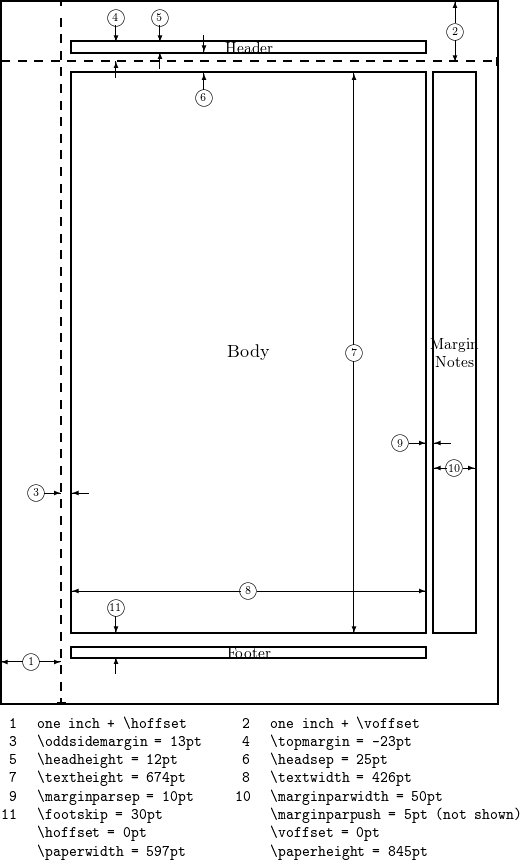
\includegraphics[height=0.8\textheight]{layout.png}
  \caption{More options for Page layout}\label{pageLayoutFig}
\end{figure}

%\begin{thebibliography}{99}
%\bibitem{datta/17}
%  Dilip Datta,\textit{\LaTeX{} in $24$ Hours. A Practical Guide for Scientific Writing}, Springer, Cham,2017
%
%\end{thebibliography}



\end{document}
%%%%%%%%%%%%%%%%%%%%%%%%%%%%
% https://www.math.uaic.ro/~maticiuc/didactic/LaTeX_Course.pdf @line 85
Left at Tables
Left lab 9-10

Add itemize....

PRINT this

ALSO PRINT Barem & checklist

Page 18 (actual 20) - dotfill
